\chapter{Particles I (Theory)} % (fold)
\label{cha:particles I (Theory)}
\section{Introduction} % (fold)
\label{sec:introduction}
接下来我们将从抽象的系综理论过渡到具体的粒子构成的系统。相当于讨论系综理论的应用。

在开始讨论之前值得稍微区分的概念是关联\index{关联}(correlation)和相互作用\index{相互作用}(interacton)。相互作用一般会涉及到力和能量,可以被写进哈密顿量,关联指的是相互之间的一种关系,是比相互作用更大的概念,比如由于泡利不相容原理带来的两个电子不能具有完全相同的量子数,不能被写进哈密顿量。

\subsection{无关联系统} % (fold)
\label{sub:无关联系统}
我们先来讨论一下粒子之间无关联的情形,无关联,也就意味着粒子与粒子之间没有任何约束关系。显然稀薄的理想气体分子之间没有相互作用,因此是一个无关联系统。接下来我们以理想气体分子为例,讨论一下无关联系统。

我们将体积$V$分成m个格子,由于气体充分地稀薄,我们可以认为每个格子中至多有一个粒子,每个格子上粒子的占据数记为$n_i$,因此\begin{equation}
    n_i=0,1.
\end{equation}
因此每一组$\{n_i\}$就对应于一个微观态。
粒子总数$N$满足\begin{equation}
    N=\sum_i^m n_i.
\end{equation}
因此就有\begin{equation}
    \braket{N}=\sum_i^m \braket{n_i}.
\end{equation}
而\begin{equation}
    \braket{(\Delta N)^2} =\braket{N^2}-\braket{N}^2
\end{equation}
注意到\begin{equation}
    N^2=\sum_i^m \sum_j^m n_i n_j.
\end{equation}
所以 \begin{equation}
    \braket{N^2}= \sum_i^m \sum_j^m \braket{n_i n_j}.
\end{equation}
考虑理想气体分子之间的无关联性,因此\begin{equation}
    \braket{n_i n_j}= \braket{n_i}\braket{n_j} \quad \text{for}\ i\neq j.
\end{equation}
进而我们就有\begin{equation}
    \begin{aligned}
        \braket{(\Delta N)^2} & =\sum_i^m \sum_j^m \braket{n_i n_j}-\sum_i^m \sum_j^m \braket{n_i}\braket{n_j} \\
                              & =\sum_i^m  \braket{n_i^2}-\sum_i^m \braket{n_i}^2                              \\
    \end{aligned}
\end{equation}
注意到$n_i^2=n_i=1$,因此就有 \begin{equation}
    \begin{aligned}
        \braket{(\Delta N)^2} & =\sum_i^m  \braket{n_i}-\sum_i^m \braket{n_i}^2 \\
                              & =\sum_i^m  \braket{n_i}(1- \braket{n_i})        \\
    \end{aligned}
\end{equation}
考虑到气体比较稀薄,因此\begin{equation}
    \braket{n_i}\ll 1.
\end{equation}
从而\begin{equation}
    \braket{(\Delta N)^2}= \sum_i^m  \braket{n_i}(1- \braket{n_i})    \approx \sum_i^m  \braket{n_i}=\braket{N}.
\end{equation}
于是对于无关联理想气体就有\begin{equation}
    \braket{N}=\braket{(\Delta N)^2} =\diffp*{{\braket{N}}}{{(\beta \mu)}}{\beta,V}
\end{equation}
在巨正则系综中,$T$和$V$固定,理想气体的密度可以表示为\begin{equation}
    \rho=\frac{\braket{N}}{V}.
\end{equation}
因此\begin{equation}
    \diffp*{{\rho}}{{(\beta \mu)}}{\beta,V} =\rho
\end{equation}
由热力学结论\begin{equation}
    \di \mu =\frac{V}{N} \di p=\frac{\di \rho}{\rho}
\end{equation}
因此\begin{equation}
    \rho=\diffp{p}{\mu}=\diffp{\rho}{{\beta \mu}}
\end{equation}
因此\begin{equation}
    \beta \diffp{p}{\rho}=1
\end{equation}
积分可以得到\begin{equation}
    \frac{p}{k_B T}=\rho+C
\end{equation}
容易验证$C=0$,于是我们就得到了理想气体状态方程\begin{equation}
    pV=Nk_BT
\end{equation}
于是立足于无关联假设和一点巨正则系综的结论,我们就可以导出理想气体状态方程。
特别地,利用
\begin{equation}
    \diffp*{{\rho}}{{(\beta \mu)}}{\beta,V} =\rho
\end{equation}
可以直接积分得到化学势的表达式\index{化学势}\begin{equation}
    \beta \mu =\ln \rho +C(T,V)
\end{equation}
因此\begin{equation}
    \mu=kT\ln p +C_1(T,V)
\end{equation}
设\begin{equation}
    \mu^{\ominus} =kT\ln p^{\ominus} +C_1(T,V)
\end{equation}
于是\begin{equation}
    \mu =\mu^\ominus +kT \ln \frac{p}{p^\ominus}
\end{equation}
% subsection 无关联系统 (end)
\subsection{配分函数因子化} % (fold)
\label{sub:配分函数因子化}
我们以最简单的正则配分函数为例\begin{equation}
    Q=\sum_v e^{-\beta \mu_v}
\end{equation}
假设每个微观态的能量都可以被分为若干不可区分且独立无关联的部分\begin{equation}
    E_v =\sum_i E_{vi}
\end{equation}
这个时候每一个微观态其实就对应于一组$\{vi\}$,因此\begin{equation}
    Q=\sum_{\{vi\}} \exp{(-\beta \sum_i E_{vi})}=\prod_i \sum_{v_i} \exp{(-\beta E_{vi})}
\end{equation}
也可以写作\begin{equation}
    Q=\prod_i Q_i
\end{equation}
其中$\displaystyle Q_i=\sum_{vi}e^{-\beta E_{vi}}$。
某一个微观态出现的概率也可以按照\begin{equation}
    p_v=\frac{e^{-\beta \mu_v}}{Q}= \frac{\prod_i e^{-\beta E_{vi}}}{\prod_i Q_i}=\prod_i p_{vi}
\end{equation}
我们刚才求积的过程就是配分函数因子化\index{配分函数因子化}。从配分函数的因子化出发,我们可以分解系综平均和涨落。

基于这些结论我们就可以来分析一个实际的$N$粒子系统。

% subsection 配分函数因子化 (end)
\subsection{全同粒子} % (fold)
\label{sub:全同粒子}
$N$个粒子的能级可以直接拆分开来\begin{equation}
    E_v=\sum_{i=1}^N E_{vi}
\end{equation}
于是\begin{equation}
    Q=Q_1^N
\end{equation}
其中单粒子的配分函数为\begin{equation}
    Q_1=\sum_{v_1} e^{-\beta E_{v_1}}=\sum_j g_j e^{-\beta E_j}
\end{equation}
但是考虑到粒子的全同性,以及稀薄假设:态的数目远远大于粒子数,两个粒子不会基本占据同一个态。因此就有\begin{equation}
    Q=\frac{Q_1^N}{N!}
\end{equation}
% subsection 全同粒子 (end)
% section introduction (end)
\section{量子统计理论} % (fold)
\label{sec:量子统计理论}
\subsection{Bose-Einstein统计和Fermi-Dirac统计} % (fold)
\label{sub:Bose-Einstein统计和Fermi-Dirac统计}
从量子力学的角度出发,全同性原理可以被表述成,交换任意两个全同粒子,其波函数在空间中的概率密度分布不会改变,也就是\begin{equation}
    |\hat{P}_{12}\psi(1,2)|^2=|\psi(1,2)|^2=|\psi(2,1)|^2
\end{equation}
因此$\hat{P}_{12}$的本征值应该是$\pm 1$。当$\psi(1,2)=\psi(2,1)$的时候,我们称之为玻色子,当$\psi(1,2)=-\psi(2,1)$的时候,我们称之为费米子。费米子满足Pauli不相容原理\index{Pauli不相容原理}:两个全同的费米子不能处于完全相同的量子态,于是对于玻色子,其某一个能级的占据数$n_k$可能是$0,1,2,...$,而对于费米子,只能是$1$或者$2$。

假设不存在简并能级玻色子和费米子在0K时的能级分布如图\ref{fig:boson and fermion}所示。这个时候对于费米子而言,最高已占据的能级就是费米能级\index{费米能级}。其定义如下\begin{definition}
    假设把所有的费米子从这些量子态上移开。之后再把这些费米子按照泡利不相容原理填充在各个可供占据的量子态上,并且这种填充过程中每个费米子都占据最低的可供占据的量子态。最后一个费米子占据着的量子态 就是费米能级。
\end{definition}
\begin{figure}[h]
    \centering
    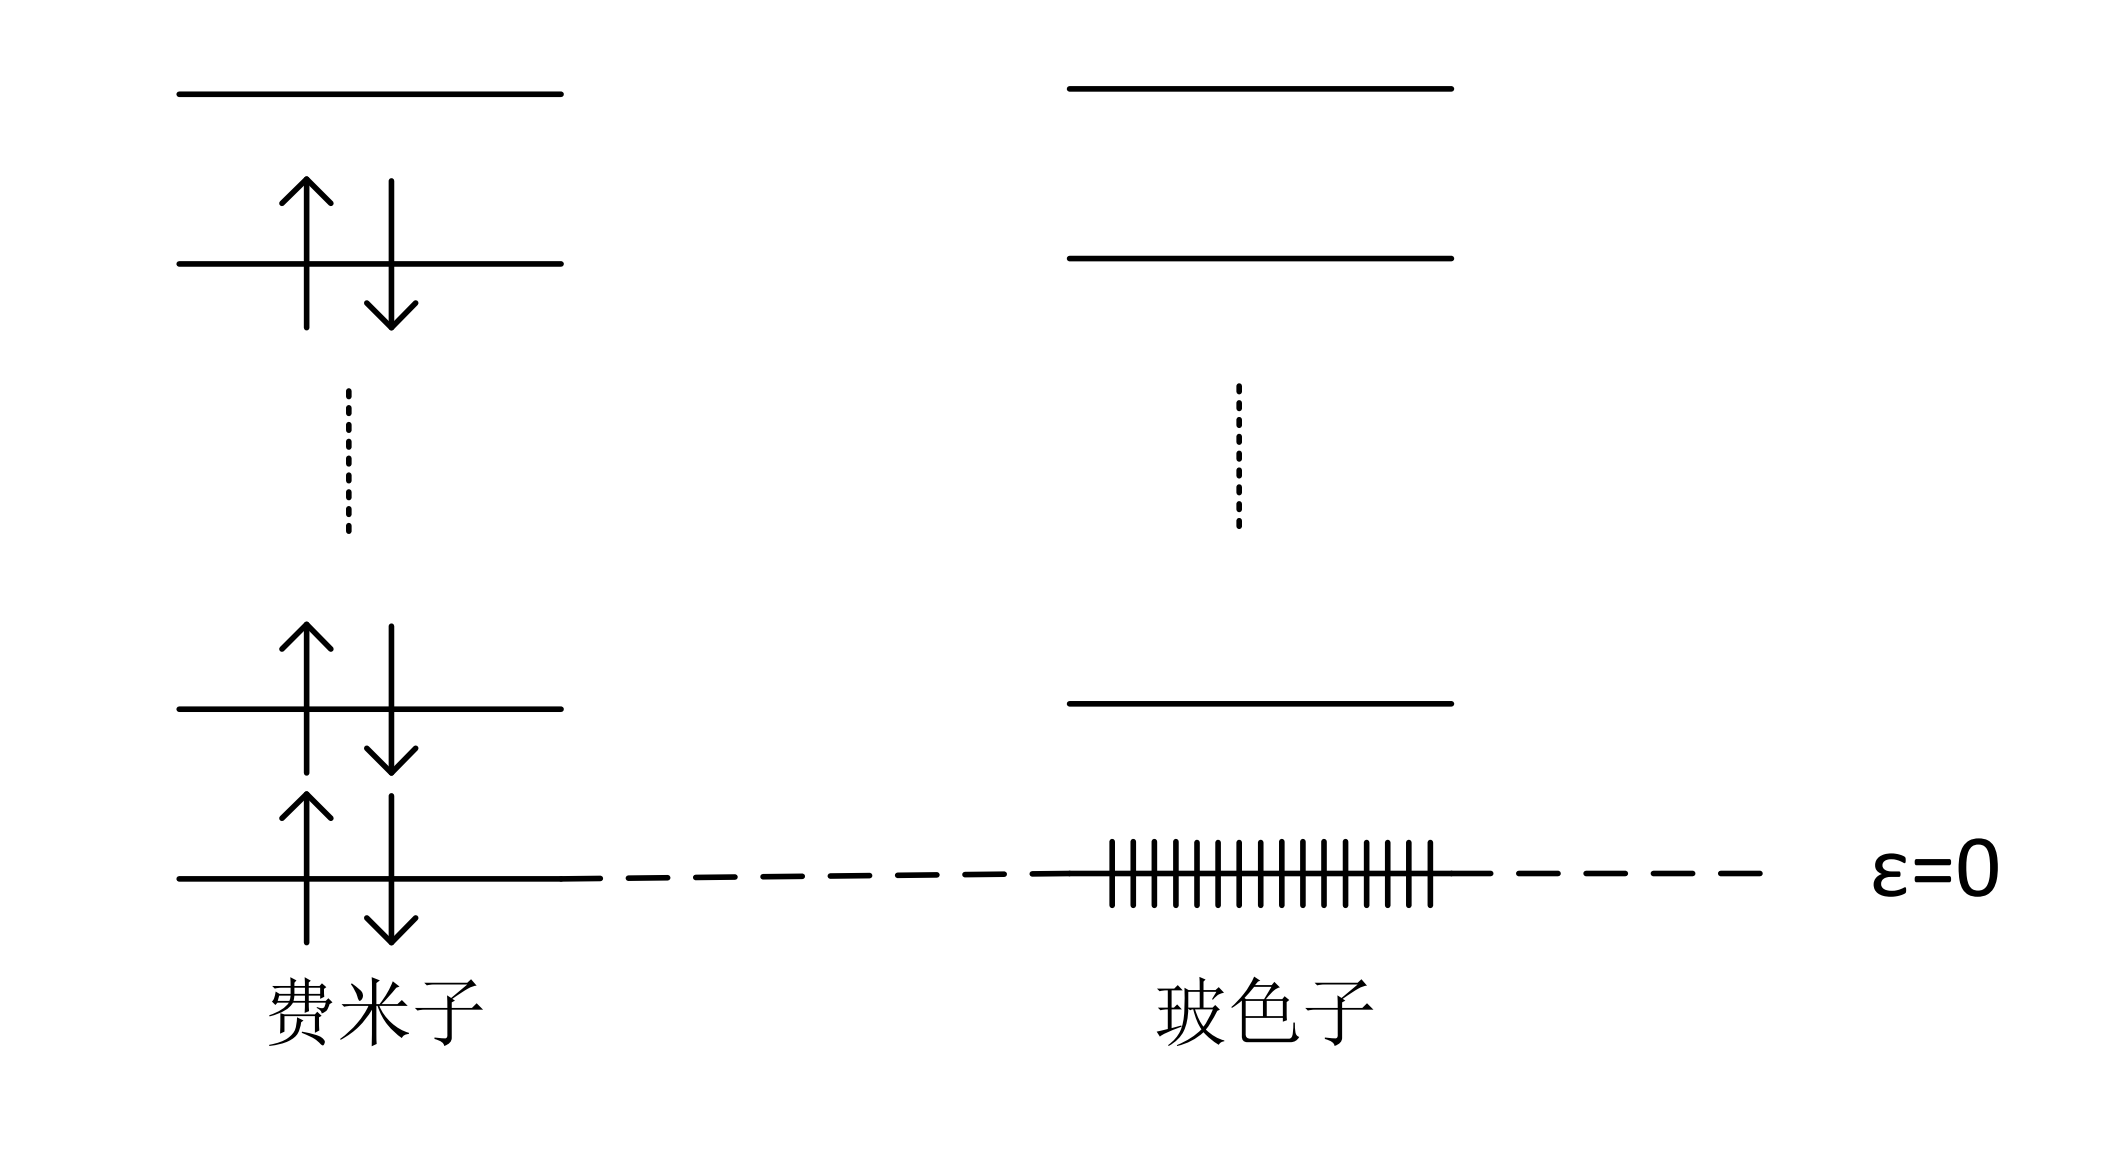
\includegraphics[width=0.64\textwidth]{fig/boson and fermion.png}
    \caption{玻色子和费米子的能级分布}
    \label{fig:boson and fermion}
\end{figure}
事实上,费米子的性质也主要由Fermi能级附近的粒子决定。

当$T>0K$的时候,粒子受热激发会跃迁到更高的未占据能级上。对于费米子,只有Fermi能级附近的粒子会受到激发,因此熵增只在很小的尺度上,而玻色子则会有宏观量级的粒子受到激发,随着温度的上升,玻色子的熵会快速增加。考虑化学势\begin{equation}
    \mu =\diffp*{E}{N}{S,V}
\end{equation}
低温情形下,对费米子新的粒子加入到费米能级附近,熵和体积都几乎不变,因此\begin{equation}
    \mu \sim E_F
\end{equation}
而对于玻色子新的粒子加入进来,就会有熵增,如果要维持熵不变,那么就需要降低体系的温度,因此保持$S$不变$N$增大,体系的能量会变小,于是\begin{equation}
    \mu = \diffp*{E}{N}{S,V}< 0
\end{equation}
在高温情形下,费米子和玻色子的熵都会随着体系的粒子数增加而增加,因此\begin{equation}
    \mu = \diffp*{E}{N}{S,V}< 0
\end{equation}

现在我们再回到统计力学的研究框架下,我们使用巨正则系综,令体系的$k$能级上的粒子占据数为$n_k$,于是粒子数\begin{equation}
    N_v=\sum_{k} n_k
\end{equation}
所以配分函数满足\begin{equation}
    \Xi =\sum_v e^{-\beta (E_v -\mu N_v)}=\sum_{\{n_k\}} e^{-\beta \sum_k n_k E_k +\beta \mu \sum_k n_k}=\sum_{\{n_k\}}\left[ \prod_k \left(e^{-\beta(\varepsilon_k-\nu)}\right)^{n_k}\right]
\end{equation}
求和和连乘可以交换,于是\begin{equation}
    \Xi =\prod_{k} \left[\sum_{n_k} \left(e^{-\beta(\varepsilon_k-\mu)}\right)^{n_k}\right] =\prod_k \Xi_k
\end{equation}
于是一个微观态的概率为\begin{equation}
    p_v =p_{\{n_k\}}=\frac{e^{-\beta (E_v -\mu N_v)}}{\Xi}=\frac{\prod_k e^{-\beta(\varepsilon_k-\mu)n_K}}{\prod_k\Xi_k}=\prod_k p_{n_k}
\end{equation}
于是原本\textbf{求体系的巨配分函数的工作就变成了求某一个状态的配分函数}。这就要简单了很多。对于费米子,$n_k$只能取$0$或者$1$,因此\begin{equation}
    \Xi_k=1+e^{-\beta(\varepsilon_k-\mu)}
\end{equation}
对于玻色子,$n_k$可以取$0,1,2,...$,因此\begin{equation}
    \Xi_k=\sum_{n_k=0}^{\infty} e^{-\beta(\varepsilon_k-\mu)n_k}=\frac{1}{1-e^{-\beta(\varepsilon_k-\mu)}}
\end{equation}
于是巨配分函数可以表示为\begin{equation}
    \Xi =\prod_k \Xi_k=\prod_k \left[1-e^{-\beta(\varepsilon_k-\mu)}\right]^{\pm 1}
\end{equation}

在此基础上,我们可以考量一个态的\textbf{平均占据数}\index{平均占据数},即\begin{equation}
    \langle n_k\rangle =\sum_{n_k} n_k p_{n_k}=\sum_{n_k} n_k \frac{e^{-\beta n_k (\varepsilon_k-\mu)}}{\Xi_{k}}=-\frac1\beta \frac{\partial \ln \Xi_k}{\partial \varepsilon_k}
\end{equation}
对于费米子这个结果为\begin{equation}
    \langle n_k\rangle =\frac{1}{e^{\beta(\varepsilon_k-\mu)}+1}
\end{equation}
对于玻色子,结果为\begin{equation}
    \langle n_k\rangle =\frac{1}{e^{\beta(\varepsilon_k-\mu)}-1}
\end{equation}

我们已经分析了占据数的系综平均,接下来我们稍微看一下占据数的涨落$\braket{(\Delta n_k)^2}$。首先我们考虑$\braket{\Delta n_k \Delta n_k'}$\begin{equation}
    \begin{aligned}
        \braket{\Delta n_k \Delta n_{k'}} & =\braket{(n_k-\braket{n_k})(n_{k'}-\braket{n_{k'}})} \\
        & =\braket{n_k n_{k'}}-\braket{n_k}\braket{n_{k'}}  \\
        & = \frac{1}{\beta^2}\left( \frac{1}{\Xi}\diffp{\Xi}{{\varepsilon_k }{\varepsilon_{k'}}} -\frac{1}{\Xi^2} \diffp{\Xi}{{\varepsilon_k}}\diffp{\Xi}{{\varepsilon_{k'}}}\right)\\
        & = \frac{1}{\beta^2}\diffp{}{{\varepsilon_k}}\left(\frac{1}{\Xi} \diffp{\Xi}{{\varepsilon_{k'}}}\right)\\
        & = \frac{1}{\beta^2}\diffp{\ln \Xi}{{\varepsilon_k }{\varepsilon_{k'}}}\\
        & = -\frac{1}{\beta}\diffp{{\braket{n_k}}}{{\varepsilon_{k'}}}
        =\begin{cases}
            0 & k\neq k' \\
            \braket{(\Delta n_k)^2} & k=k'
        \end{cases}
    \end{aligned}
\end{equation}
于是占据数的涨落为\begin{equation}
\begin{aligned}
    \braket{(\Delta n_k)^2}& =-\frac{1}{\beta}\diffp{{\braket{n_k}}}{{\varepsilon_{k}}} =-\frac{1}{\beta}\diffp{{(e^{\beta (\varepsilon_k-\mu)}\pm 1)^{-1}}}{{\varepsilon_{k}}} 
    & = \frac{e^{\beta (\varepsilon_k-\mu)}}{( e^{\beta (\varepsilon_k-\mu)}\pm 1)^{2}}=\braket{n_k}\mp \braket{n_k}^2
\end{aligned}\end{equation}

事实上对于费米子而言这个结果是比较显然的,因为$n_k=0,1$,所以$n_k^2=n_k$\begin{equation}
    \braket{n_k^2}-\braket{n_k}^2=\braket{n_k}-\braket{n_k}^2
\end{equation}

现在我们对我们前面得到的结论稍微做一点分析,比如平均占据数\begin{equation}
    \langle n_k\rangle =\frac{1}{e^{\beta(\varepsilon_k-\mu)}\pm 1}
\end{equation}
对于费米子,\begin{equation}
    \langle n_k\rangle =\frac{1}{e^{\beta(\varepsilon_k-\mu)}+1}
\end{equation}
显然$0\le \braket{n_k}\le 1$,当且仅当$T=0$K的时候,可以取到等号,此时\begin{equation}
    \braket{n_k}=\begin{cases}
        0 & \varepsilon_k>\mu \\
        1 & \varepsilon_k<\mu
    \end{cases}
\end{equation}
当$\varepsilon_k=\mu$的时候,$\braket{n_k}=\frac{1}{2}$,所以我们可以进一步的了解前面提到的费米能级:费米能级以下平均占据数都为1,以上占据数都为0,费米能级自己的平均占据数为$\frac{1}{2}$。

对于玻色子
\begin{equation}
    \braket{n_k}=\frac{1}{e^{\beta(\varepsilon_k-\mu)}-1}
\end{equation}
考虑到$\braket{n_k}$的物理意义,因此$\varepsilon_k\le \mu$恒成立。到这里,我们已经基本完成了对量子统计理论的讨论,接下来我们开始讨论经典统计的方法。
% subsection Bose-Einstein统计和Fermi-Dirac统计 (end)
\subsection{经典极限} % (fold)
\label{sub:经典极限}
经典统计最基本的认知就是前面讨论的:态的数目远远大于粒子的数目,完成了前面的讨论之后,我们有一种等价的说法$\braket{n_k}\ll 1$。

当$\braket{n_k}\ll 1$的时候,也就有$e^{\beta (\varepsilon_k-\mu)}\gg 1$,因此我们就有\begin{equation}
    \braket{n_k}=\frac{1}{e^{\beta(\varepsilon_k-\mu)}\pm 1}\approx e^{-\beta(\varepsilon_k-\mu)}
\end{equation}
这就是经典极限下的Maxwell-Boltzman分布。注意到此时\begin{equation}
    \braket{n_0} =e^{\beta \mu} \ll 1
\end{equation}
这也就是经典统计\index{经典统计}的一种等价说法,$e^{\beta \mu} \ll 1$,即$\mu$是一个绝对值很大的负数。

对于上述的Maxwell-Boltzman分布,我们有\begin{equation}
    \braket{N}=\sum_{k} \braket{n_k}=e^{\beta \mu} \sum_{k} e^{-\beta\varepsilon_k}=qe^{\beta \mu}
    \label{equ:N with exp beta mu}
\end{equation}
其中$q$为单粒子配分函数。因此\begin{equation}
    \frac{\braket{N}}{q}=e^{\beta \mu} \ll 1
\end{equation}
这就又是经典统计的等价表述:单粒子的配分函数远远大于粒子总数。其中,粒子处于状态$k$的概率为\begin{equation}
    p_k =\frac{\braket{n_k}}{\braket{N}}=\frac{e^{-\beta \varepsilon_k}}{q}
\end{equation}
这个结果和热力学中的结论是一致的。

% subsection 经典极限 (end)
\subsection{巨正则系综的应用} % (fold)
\label{sub:巨正则系综的应用}
介绍了两种统计方法之后,我们再回到巨正则系综的理论中来。考察一个多组分的体系,有\begin{equation}
\begin{aligned}
    \Xi &=\sum_v e^{\beta (\sum_i \mu_i N_i^v -E_v)}\\
    &=\sum_{\{N_i\}} e^{\beta \sum_i N_i} \sum_{N_i^v=N_i} e^{-\beta E_v} \\
    &=\sum_{\{N_i\}} e^{\beta \sum_i N_i} Q(T,V,N_i)
\end{aligned}
\end{equation}
取最概然近似,就有\begin{equation}
    \Xi \approx e^{\beta \sum_i \mu_i\braket{N_i}} Q(T,V,\braket{N_i})
\end{equation}
于是可以得到\begin{equation}
    \ln Q =\ln \Xi -\beta \sum_i \mu_i\braket{N_i}
    \label{equ:Q with Xi}
\end{equation}

另一方面,对一个粒子系统,有\begin{equation}
    N_i^v =\sum_{k_i} n_{k_i},\quad E^v=\sum_i\sum_{k_i}n_{k_i} \varepsilon_{k_i}
\end{equation}
代入巨正则系综配分函数的表达式可以得到\begin{equation}
   \begin{aligned}
    \Xi &=\sum_{\{n_{k_i}\}} e^{\sum_i\sum_{k_i}\beta(\mu_i-\varepsilon_{k_i})n_{k_i} } \\
    & = \prod_i \prod_{k_i} \left[\sum_{n_{k_i} }e^{\beta(\mu_i-\varepsilon_{k_i})n_{k_i} }\right]
    &= \prod_i \prod_{k_i} \left[1\pm e^{\beta(\mu_i-\varepsilon_{k_i})n_{k_i} }\right]
   \end{aligned}
\end{equation}
因为$e^{\beta (\mu_i -\varepsilon_{k_i})}\ll1$,利用当$x\to 0$的时候$\ln (1\pm x)\sim pm x$,于是\begin{equation}
    \ln \Xi \approx \sum_i \sum_{k_i} e^{\beta(\mu_i-\varepsilon_{k_i})}
\end{equation}
代入式\ref{equ:Q with Xi},我们就可以得到\begin{equation}
\begin{aligned}
    \ln Q &= \sum_i \sum_{k_i} e^{\beta(\mu_i-\varepsilon_{k_i})}- \beta \sum_i \mu_i\braket{N_i}
    &=\sum_i e^{\beta \mu_i} q_i - \beta \sum_i \mu_i\braket{N_i}\\
    &=\sum_i \left(e^{\beta \mu_i} q_i -\beta \mu_i\braket{N_i}\right)
    \label{equ:Q with exp beta mu qi and N}
\end{aligned}
\end{equation}
由式\ref{equ:N with exp beta mu},我们知道\begin{equation}
    e^{\beta \mu_i}=\frac{\braket{N_i}}{q_i}\ \Rightarrow \  \beta \mu_i =\ln\braket{N_i} -\ln q_i
\end{equation}
代入\ref{equ:Q with exp beta mu qi and N},我们可以得到\begin{equation}
    \begin{aligned}
        \ln Q &=\sum_i \left(\braket{N_i} -\braket{N_i}\ln \braket{N_i} +\braket{N_i}\ln q_i\right)\\
        & \approx \sum_i \left(\ln q_i^{N_i}-\ln N_i!\right)\\
        &=\sum_i \ln \frac{q_i^{N_i}}{N_i!}
    \end{aligned}
\end{equation}
也即\begin{equation}
    Q =\prod_i \frac{q_i^{N_i}}{ \ln N_i!}
\end{equation}
% subsection 巨正则系综的应用 (end)

% section 量子统计理论 (end)
\begin{review}
    \item 无关联系统的统计理论
    \item 配分函数因子化;
    \item 全同粒子;
    \item Bose-Einstein统计;
    \item Fermi-Dirac统计;
    \item 量子统计的经典极限;
    \item 巨正则系综的应用
\end{review}
\section{习题} % (fold)
\label{sec:习题4}

% section 习题 (end)
% chapter particles I (Theory) (end)


%---------------------------------------------------------------------------